\chapter{Hydrate layers and particle distances}
\label{chap:hydrate-rim}

\textit{Some of the results and data presented in this chapter have already been published in \cite{kleiner.2024a}. However, the datasets were significantly extended and re-evaluated.}

The methods presented in \zcref{subsec:algo_hlm, sec:ebsd-hydrate} were applied to pure hydrated \ac{C3S} and \ac{C2S} specimens as well as mixtures of both phases at different ages, which were embedded, polished, and coated with carbon.
The datasets differ in the imaged area and slightly in \ac{SEM} imaging parameters.
For example, the accelerating voltage used varied from \qtyrange{10}{15}{\kilo\volt}.
The raw images are publicly available \cite{kleiner.2023a, kleiner.2025e, kleiner.2025d}.
Furthermore, the method was adapted to measure particle distances and was combined with \ac{EBSD} measurements.
However, the methods first had to be validated.

\section{Validation of algorithms}
\label{sec:ebsd-hydrate-validation}

To validate the algorithms introduced in \zcref{sec:ebsd-hydrate,subsec:algo_hlm}, simulated datasets were created.
For this purpose, an artificial volume was randomly filled with \num{120000} spherical \ac{C3S} particles per \unit{\cubic\milli\meter}.
A \textsc{Gaussian} distribution of particle diameters was generated with diameters ranging from $d_\text{min, \ac{C3S}}=$\qty{0}{\micro\meter} to $d_\text{max, \ac{C3S}}=$\qty{5}{\micro\meter} was selected. 
The total volume was set to \qtyproduct{2000x2000}{\micro\meter\squared} with a height ($z$) of four times the maximum diameter of a hydrated \ac{C3S} grain.
The simulation allows the \ac{HLT} to be varied depending on the crystal orientation of the clinker grains.
To enable this, a random crystal orientation was assigned to each \ac{C3S} grain (based on the monoclinic unit cell \acs{ICSD} 94742 \cite{delatorre.2002}).
Two scenarios were then created for validation.
For the validation of the \ac{HLT} measurement algorithm, a constant spherical hydrate layer was used.
To validate the \ac{EBSD} correlation, the hydrate layer was modelled as an ellipsoid whose orientation varied according to the assigned crystal orientation.

Slicing this volume, generated a virtual \ac{BSE} image (\qty{0.2}{\micro\meter\per\px}), which was then be used as input for the methods to be validated.
Sections of such synthetic \ac{BSE} images are shown in \zcref{fig:c3s_synthetic_BSE}.

\begin{figure}[htb!]
    \centering

    \begin{subfigure}[t]{0.49\linewidth}
        \includegraphics[width=\textwidth,trim={0 0 0 1cm},clip]{hydrate-rim/ebsd/evaluation/synthetic_bse_slice_round.pdf}
        \caption{Spherical hydrate layer.}
    \end{subfigure}%
    \hfill%
    \begin{subfigure}[t]{0.49\linewidth}

        \includegraphics[width=\textwidth,trim={0 0 0 1cm},clip]{hydrate-rim/ebsd/evaluation/synthetic_bse_slice_eliptic.pdf}
        \caption{Ellipsoidal hydrate layer.}
    \end{subfigure}%
        
        \caption{
            Examples of synthetically generated \ac{BSE} images with a spherical \qty{2}{\micro\meter} hydrate layer (left) and an ellipsoidal hydrate layer with semi-axes of \qtyproduct{0.5x3.0x5}{\micro\meter} (right).
            The red lines depict the selected hydrate layer thicknesses.
            Black: porosity; dark grey: \ac{CSH}; light grey: \ac{C3S}.
        }
    \label{fig:c3s_synthetic_BSE}
\end{figure}

Applying the \ac{HLT} measurement to the synthetic \ac{BSE} images results in \zcref{fig:c3s_synthetic_BSE_HLT}.
The diagrams consist of a graph indicating frequency of a measured \ac{HLT} as a function of the grain size (blue-green).
This plot is accompanied by a frequency plot of the grain size diameter (grey) and a grain-size-agnostic distribution plot of the \ac{HLT} frequency (orange).
The set values for the respective \ac{HLT} are marked with red lines.

\begin{figure}[htb!]
    \centering

    \includegraphics[width=\textwidth]{hydrate-rim/ebsd/evaluation/2D_cir_vs_elliptic.pdf}
        
    \caption{
        Normalised distributions of the \ac{HLT} of simulated hydrated \ac{C3S} depending on the particle diameter; 
        left: spherical hydrate layer (\qty{3}{\micro\meter}); right: ellipsoidal hydrate layer (\qtyproduct{0.5x3.0x5}{\micro\meter}).
        The histogram (grey) on top illustrates the logarithmic frequency for each diameter bin in the diagram below.
        The histogram (orange) on the right illustrates the frequency of \ac{HLT} measurements as the sum of the main diagram.
    }
    \label{fig:c3s_synthetic_BSE_HLT}
\end{figure}

The diagrams are distinctly different.
The spherical hydrate layer results in a fairly constant \ac{HLT} with a maximum at \qty{3.3}{\micro\meter}.
This value is \qty{10}{\percent} higher than the simulated layer thickness.
While one reason for this overestimation is the sectioning effect (see \zcref{subsec:sectioning-effect}), another reason is the merging of the hydrate layers of multiple grains, causing a larger \ac{HLT} for some measurements.
The simulated elliptical hydrate layer shows a much broader distribution of the \ac{HLT}.
The maximum value of the \ac{HLT} was measured at \qty{2.9}{\micro\meter}, but the majority of measurements are distributed between the set limits for the ellipsoid.

For both measurements, the data density below a grain diameter of \qty{4}{\micro\meter} was low.
However, these smaller grains seem to have a tendency to larger \ac{HLT}s, which can also be explained with the sectioning effect.
In real specimens, many more smaller grains are expected than in this simulation, changing the appearance of the distribution for smaller grains.
Finally, the 2D plot and the grain diameter histogram show regular vertical artefacts, which are probably caused by rounding errors, but do not affect the evaluation and are less pronounced in real-world data.

Using the assigned crystal orientations, a simulated \ac{EBSD} dataset was generated with a resolution of \qty{2}{\micro\meter\per\px} in the form of a channel text file.
The resolution of the simulated \ac{BSE} image only had to be adjusted to the \ac{EBSD} dataset, since the datasets were already aligned to each other.
After processing the data as explained in \zcref{sec:ebsd-hydrate}, the \ac{HLT} measurements can be projected onto a unit sphere representing the crystal orientation of \ac{C3S} (see \zcref{fig:ebsd_eval_sphere}).

\begin{figure}[htb!]
	\centering
    
    \begin{subfigure}[t]{0.49\linewidth}
        \begin{tikzpicture}
            \begin{axis}[
                width=0.66\textwidth,
                height=0.66\textwidth,
                scale only axis,
                enlargelimits=false,
                xmin=-1.1, xmax=1.1,
                ymin=-1.1, ymax=1.1,
                axis on top,
                colormap name=magma,
                colorbar,
                colorbar style={
                    ylabel={\ac{HLT} in \unit{\micro\meter}},
                },
                point meta min=0,
                point meta max=12.1,
                ticklabel style={font=\small},
                xtick={-1,0,1},
                ytick={-1,0,1},
            ]
                \addplot [draw=none] coordinates {(-1,-1) (1,1)};
                \node[inner sep=0pt, anchor=south west] at (axis cs:-1,-1) {
                    \ifdefined\PRINTABLE
                        \includegraphics[width=0.6\textwidth]{hydrate-rim/ebsd/evaluation/ani_scatter/scatter00.jpg}
                    \else
                        \animategraphics[loop,autoplay,width=0.6\textwidth]{12}{hydrate-rim/ebsd/evaluation/ani_scatter/scatter}{00}{35}
                    \fi
                };
            \end{axis}
        \end{tikzpicture}
        \caption{
            \ac{HLT} scatter plot on a unit sphere..
            \label{fig:ebsd_eval_sphere_a}
        }
    \end{subfigure}%
    \hfill%
    \begin{subfigure}[t]{0.49\linewidth}
        
        \begin{tikzpicture}
            \begin{axis}[
                width=0.66\textwidth,
                height=0.66\textwidth,
                scale only axis,
                enlargelimits=false,
                xmin=-1.1, xmax=1.1,
                ymin=-1.1, ymax=1.1,
                axis on top,
                colormap name=magma,
                colorbar,
                colorbar style={
                    ylabel={\ac{HLT} in \unit{\micro\meter}},
                },
                point meta min=0,
                point meta max=4.07,
                xtick={-1,0,1},
                ytick={-1,0,1},
                ticklabel style={font=\small},
            ]
                \addplot [draw=none] coordinates {(-1,-1) (1,1)};
                \node[inner sep=0pt, anchor=south west] at (axis cs:-1,-1) {
                    
                    \ifdefined\PRINTABLE
                        \includegraphics[width=0.6\textwidth]{hydrate-rim/ebsd/evaluation/ani_healpix/healpix04.jpg}
                    \else
                        \animategraphics[loop,autoplay,width=0.6\textwidth]{12}{hydrate-rim/ebsd/evaluation/ani_healpix/healpix}{35}{00}
                    \fi
                    
                };
            \end{axis}
        \end{tikzpicture}
        \caption{
            Mean \ac{HLT} in a \textsc{HEALPix} grid on a unit sphere.
            \label{fig:ebsd_eval_sphere_b}
        }
    \end{subfigure}
    
	\caption{
        Unit sphere indicating \ac{HLT} measurements corresponding to the crystal orientation of a simulated \ac{C3S} dataset with an elliptical hydrate layer (\qtyproduct{0.5x3.0x5}{\micro\meter}) in a scatter plot (a) and in a \ac{HEALPix} grid (b).
        \label{fig:ebsd_eval_sphere}
    }
\end{figure}

Since the measurement density is not very high, the unit sphere was divided into a so-called \ac{HEALPix} grid \cite{gorski.2005}.
In a \ac{HEALPix} grid, the surface of the sphere is divided into sections of equal area.
This avoids a statistical distortion, especially at the poles of the unit sphere.
The mean \ac{HLT} within each \ac{HEALPix} grid cell was calculated and each cell was coloured accordingly (see \zcref{fig:ebsd_eval_sphere_b}).

If there is a dependence between the crystal orientation and the \ac{HLT}, it should become visible as a concentration of longer or shorter \ac{HLT}s in certain areas of the unit sphere.
Additionally, for an ideal preparation a homogeneous distribution of measurement counts is expected around the unit sphere.
While it becomes apparent for the elliptical hydration rim simulation, that the \ac{HLT} distribution is not uniform in \zcref{fig:ebsd_eval_sphere_b}, a \textsc{Mollweide} projection of the whole sphere surface is shown in \zcref{fig:ebsd_eval_sphere_projection}.

\begin{figure}[htb!]
	\centering
    \begin{subfigure}[t]{0.49\linewidth}
        
        \begin{tikzpicture}
            \begin{axis}[
                width=.8\textwidth,
                height=.45\textwidth,
                scale only axis,
                enlargelimits=false,
                colormap name=magma,
                colorbar,
                colorbar style={
                    ylabel={Average \ac{HLT} in \unit{\micro\meter}},
                    font=\small
                },
                point meta min=0,
                point meta max=4.07,
                xtick={-1,0,1},
                ytick={-1,0,1},
                ticklabel style={font=\footnotesize},
                hide axis,
            ]
                \addplot [draw=none] coordinates {(-1,-1) (1,1)};
                \node[inner sep=0pt, anchor=south west] at (axis cs:-1,-1) {
                    
                \includegraphics[width=.8\textwidth]{hydrate-rim/ebsd/evaluation/ellipsoid_mollweide_len.png}
                    
                };
            \end{axis}
        \end{tikzpicture}
        
        \caption{
            Mean \ac{HLT}.
            \label{fig:ebsd_eval_sphere_projection_b}
        }

    \end{subfigure}
    \hfill
    \begin{subfigure}[t]{0.49\linewidth}
        \begin{tikzpicture}
            \begin{axis}[
                width=.8\textwidth,
                height=.45\textwidth,
                scale only axis,
                enlargelimits=false,
                hide axis,
                colormap name=ocean_r,
                colorbar,
                colorbar style={
                    ylabel={$log_{10}(n+1)$},
                    font=\small
                },
                point meta min=0,
                point meta max=2.25,
                xtick={-1,0,1},
                ytick={-1,0,1},
                ticklabel style={font=\footnotesize},
            ]
                \addplot [draw=none] coordinates {(-1,-1) (1,1)};
                \node[inner sep=0pt, anchor=south west] at (axis cs:-1,-1) {
                    
                \includegraphics[width=.8\textwidth]{hydrate-rim/ebsd/evaluation/ellipsoid_mollweide_cnt.png}
                    
                };
            \end{axis}
        \end{tikzpicture}
        
        \caption{
            Data density plot.
            \label{fig:ebsd_eval_sphere_projection_a}
        }
    \end{subfigure}
    
	\caption{
        The same \ac{HEALPix} grid as in \zcref{fig:ebsd_eval_sphere_b} is shown in a \textsc{Mollweide} projection (a), together with the corresponding data density plot (b). 
        The lines ({\color{red}red}) are a projection of the monoclinic structure of \ac{C3S} as derived from \zcref{fig:c3s_unit_cell}. % HEALPix Mollweide
        \label{fig:ebsd_eval_sphere_projection}
    }
\end{figure}

This visualisation underlines that, for the elliptical hydration rim simulation, both the inhomogeneous but symmetric \ac{HLT} distribution and the homogeneous data density distribution are present as expected.
The \textsc{Mollweide} projection from \zcref{fig:ebsd_eval_sphere_projection_b} can also be projected back to the \ac{C3S} unit cell as illustrated in \zcref{fig:c3s_eval_backprojection}.
This figure shows the unit cell in 3D and unfolded as a net, and demonstrates which crystallographic surface was set to grow the largest \ac{HLT} value in the simulation.

\begin{figure}[htb!]
    \centering

    \begin{tikzpicture}
        \begin{axis}[
            width=.87\textwidth,
            height=.27\textwidth,
            scale only axis,
            enlargelimits=false,
            hide axis,
            colormap name=magma,
            colorbar,
            colorbar style={
                ylabel={Average \ac{HLT} in \unit{\micro\meter}},
            },
            point meta min=0,
            point meta max=4.07,
            xtick={-1,0,1},
            ytick={-1,0,1},
            ticklabel style={font=\small},
        ]
            \addplot [draw=none] coordinates {(-1,-1) (1,1)};
            \node[inner sep=0pt, anchor=south west] at (axis cs:-1,-1) {
                
            \includegraphics[width=.9\textwidth]{hydrate-rim/ebsd/evaluation/healpix_meanlen_cube_net_2d+3D.pdf}
                
            };
        \end{axis}
    \end{tikzpicture}
        
    \caption{
        Projection of the unit sphere from \zcref{fig:ebsd_eval_sphere_projection} to the unit cell of \ac{C3S}, MIII polymorph.
        Left: 3D visualisation of the unit cell with the mean \ac{HLT} values on each surface.
        Right: Net of the unit cell with the projected HEALPix grid.
    }
    \label{fig:c3s_eval_backprojection}
\end{figure}

The same experiment was done for the spherical hydrate layer.
As expected, both the \ac{HLT} and the measurement density were distributed homogeneously on the unit sphere.

\section{Influence of the segmentation method}

This section benchmarks and discusses different segmentation methods on a selected specimen.
The evaluation is performed on a \qtyproduct{0.5 x 0.5}{\milli\meter\squared} section of stitched \ac{SEM}-\ac{BSE} images of \qty{14}{\day}-hydrated \ac{C3S} \cite{kleiner.2024a}.
Three different segmentation methods were applied:

\begin{enumerate}
	\item a manually selected threshold value to distinguish between pores, hydrate phases, and the unhydrated clinker,
	\item a manually trained pixel classification algorithm distinguishing between pores, the unhydrated clinker, \ac{CH}, and
	\begin{enumerate}
		\item separated inner and outer \ac{CSH},
		\item combined inner and outer \ac{CSH},
	\end{enumerate}
	\item manual segmentation, based on the pixel classification result, ignoring \ac{CSHo}.
\end{enumerate}

%Additionally, a representative area demonstrating the performed measurements is shown in the \ac{SI} of \cite{kleiner.2024}, Figure 2.
A comparison of the raw segmentation results (see \zcref{fig:results_segmentation_methods, tab:segmentation}) reveals apparent differences.
The threshold segmentation leads to many erroneously identified phases.
In contrast, the pixel classification produces a result very close to the manual segmentation.
However, if \ac{CSHo} is taken into account in the pixel classification, the \ac{HLT} distribution and the calculated $l_\text{max}$ (the most frequent \ac{HLT}) are comparable to the threshold-based segmentation, whilst the data density is significantly reduced (see \zcref{tab:segmentation} and \zcref{fig:hlt_segmentation_influence} \cite{kleiner.2024}, \ac{SI}).
This data density reduction is caused by a rough segmentation of the \ac{CSHo} and, therefore, a significantly decreased pore space.
Furthermore, a slightly larger \qty{33.3}{\percent} confidence interval and a significant reduction of the first \ac{HLT} accumulation can be observed when including the \ac{CSHo}.

\begin{figure}[p]
    \centerline{\includegraphics[width=\textwidth]{hydrate-rim/supplementary/threshold_types.pdf}}
    \caption{
		Segmentation results of \qty{14}{\day} hydrated \ac{C3S}.
        Raw image (A); segmentation result by thresholding (B), pixel classification (C) and manual segmentation (D).
		Grey: raw data; {\color{blue}blue}: \ac{C3S}; {\color{green}green}: hydrates (C and D only dense \ac{CSH}); {\color{red}red}: \ac{CH}; {\color{orange}yellow}: \ac{CSHo}.
		\cite{kleiner.2024}, \ac{SI}
	}
	\label{fig:results_segmentation_methods}
\end{figure}

\begin{figure}[p]
    \centerline{\includegraphics[width=\textwidth]{hydrate-rim/supplementary/segmentation_results.pdf}}
    \caption{
		Visualisation of the measured \ac{HLT}.
		Valid measurements are indicated in {\color{green}green} around the \ac{C3S} in {\color{blue}blue}. \ac{C3S} grains in {\color{red}red} were filtered or had not enough measurements.
		Segmentation result by thresholding (A), pixel classification with (B) and without \ac{CSHo} (C) and manual segmentation (D).
		\cite{kleiner.2024}, \ac{SI}
	}
	\label{fig:results_segmentation_methods_HLT}
\end{figure}

Thresholding results in a higher number of excluded and fewer valid measurements than the other methods.
One main reason is the presence of dense regions filled with \ac{CH}, since no phase transition between hydrate and pores is present in those areas.
Manual segmentation and pixel classification ignoring \ac{CSHo} show nearly identical $l_\text{max}$ values, while restoring the data density (see \zcref{fig:results_segmentation_methods_HLT}).

The difference in the $l_\text{max}$ of the pixel classification results allows the estimation of a \ac{CSHo} thickness of roughly \qty{0.4}{\micro\meter}.
Nevertheless, segmenting the outer layer presents a non-trivial challenge as it relies on the person performing the segmentation and training the pixel classification.
In many cases, whether \ac{CSHo} or merely an artefact such as a flat edge is being segmented remains unclear.

%An overview of the influence of the segmentation method on the results can be found in \zcref{tab:segmentation}.

\begin{table}[htbp]
	\centering
	\caption{
		Influence of the segmentation method of a cropped dataset with a reduced resolution (age: \qty{14}{\day}; image area: \qty{0.25}{\square\milli\meter}; resolution: \qty{84.3}{\nano\meter\per\px}). \cite{kleiner.2024}
		The table indicates the time required to apply the segmentation method, the measured areas, and $l_\text{max}$.
	}
	\begin{tabularx}{\textwidth}{@{}l*{4}{>{\centering\arraybackslash}X}@{}}
		\toprule
		\multirow{3}{*}{segmentation method} & 1. & 2.a & 2.b & 3. \\

																	& threshold		& \multicolumn{2}{c}{pixel classification} & manual\\
																	& {--} & w. \ac{CSHo} & wo. \ac{CSHo} & {--} \\ \midrule
		time required												& $\approx$\,\qty{5}{\minute} & \multicolumn{2}{c}{$\approx$\,\qty{4}{\hour}} & $\approx$\,\qty{2}{weeks} \\\midrule

		pores in \unit{\areapercent}								& 23.3   & 22.0   & 30.7   & 30.0 \\
		\ac{CSH} in \unit{\areapercent}								& 62.9   & 52.5   & 52.5   & 53.4 \\
		\ac{CSHo} in \unit{\areapercent}							& {--}   &  8.6   & {--}   & {--} \\
		clinker in \unit{\areapercent}								& 13.9   & 16.8   & 16.8   & 16.7 \\ \midrule
		$l_\text{\qty{-33.3}{\percent}}$ in \unit{\micro\meter}		&  1.43  & 1.43   & 1.18   & 1.18 \\
		$l_\text{max}$ in \unit{\micro\meter}						&  1.85  & 1.94   & 1.52   & 1.52 \\
		$l_\text{+\qty{33.3}{\percent}}$ in \unit{\micro\meter}		& 2.28   & 2.44   & 1.85   & 1.94 \\
		\bottomrule
	\end{tabularx}
	\label{tab:segmentation}
\end{table}

The phase composition indicates the reaction progress of the specimen.
The porosity data must be interpreted with caution and cannot be reliably evaluated, as the measurement of total porosity can be significantly influenced by the presence of air voids and cracks within the specimen.
Therefore, the hydrate content within the solids $F_\text{hydrate}$ was calculated:

\begin{equation}
	F_\text{hydrate} = \frac{A_{\text{hydrate}}}{A_{\text{clinker}} + A_{\text{hydrate}}}
\end{equation}

\zcref{fig:segmentation_hydrate_clinker_ratio} indicates the variation in $F_\text{hydrate}$ caused by different segmentation methods.

% Bar chart: Normalised hydrate content F_hydrate
% Values taken from table \ref{tab:segmentation}:
% method 1: 62.9 / (13.9 + 62.9) * 100 = 81.9
% method 2.a: 61.1 / (16.8 + 61.1) * 100 = 78.4
% method 2.b: 52.5 / (16.8 + 52.5) * 100 = 75.8
% method 3: 53.4 / (16.7 + 53.4) * 100 = 76.2
\begin{figure}[htbp]
	\centering
	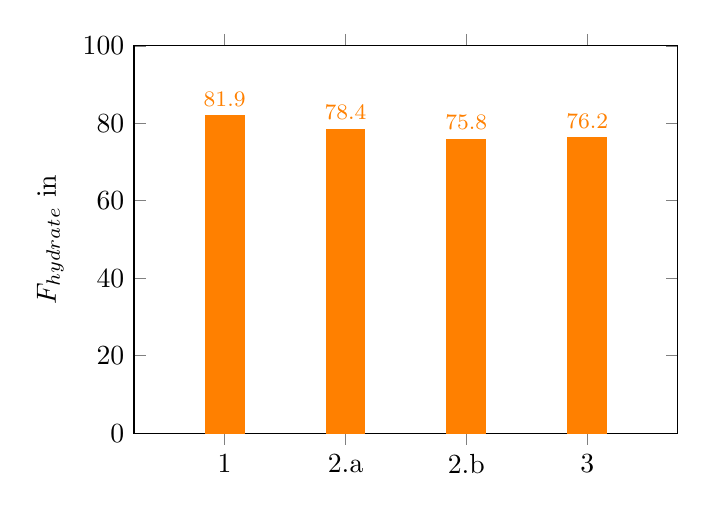
\begin{tikzpicture}
		\begin{axis}[
			ybar,
			ymin=0, ymax=100,
			ylabel={$F_\text{hydrate}$ in \unit{\percent}},
			symbolic x coords={1,2.a,2.b,3},
			xtick=data,
			enlarge x limits=0.25,
			nodes near coords,
			nodes near coords style={
				font=\footnotesize,
				/pgf/number format/.cd,
				fixed,
				precision=1
			},
			bar width=14pt,
			height=6.5cm,
			width=.7\textwidth,
		]
			\addplot+[fill=orange, orange] coordinates {(1,81.9) (2.a,78.4) (2.b,75.8) (3,76.2)};
		\end{axis}
	\end{tikzpicture}
	\caption{
		Normalised hydrate content $F_\text{hydrate}$ for various segmentation methods.
		1: threshold, 2: pixel classification (a: with and b: without \ac{CSHo}), 3: manual segmentation.
	}
	\label{fig:segmentation_hydrate_clinker_ratio}
\end{figure}

Simple thresholding overestimates the proportion of hydration products by more than \qty{5}{\percent}.
In contrast, the pixel classification (ignoring \ac{CSHo}) deviates by only \qty{2}{\percent} from the manual segmentation result.
The estimated time required to manually train this model is approximately \qty{4}{\hour}, although this can vary considerably depending on the training results.
However, the thresholding method is the fastest option.
It can perform well if the raw images have good phase contrast, which can be difficult to achieve due to the small differences in the backscatter coefficient $\eta$, as described in \zcref{sec:bse}.
In some cases, large-scale \ac{BSE} images may exhibit brightness deviations from one edge to another, or the overall brightness of image tiles within a larger image set may change (for example, due to charging).
These artefacts can significantly influence the thresholding method in particular.

\FloatBarrier
\section{Single phase analysis}

Initially, the individual phases were analysed.
The images reveal distinct differences in the morphology of the hydration products.
For example, the \ac{CSH} needles in hydrated \ac{C3S} are small and form on a dense \ac{CSHi} rim.
In contrast, hydrated \ac{C2S} produces coarser needles with a less homogeneous, dense \ac{CSH} layer underneath (see \zcref{fig:single_phase_examples}).
Furthermore, a higher number of unhydrated \ac{C2S} particles can be observed in the same area, often shattered into smaller fragments.

\begin{figure}[htb!]
    \centering

	\begin{subfigure}{0.49\textwidth}
		\includegraphics[width=\textwidth]{hydrate-rim/single_phase_C3S.pdf}
		\caption{\ac{C3S}.}
		\label{fig:single_phase_examples-alite}
	\end{subfigure}
	\hfill
	\begin{subfigure}{0.49\textwidth}
		\includegraphics[width=\textwidth]{hydrate-rim/single_phase_C2S.pdf}
		\caption{\ac{C2S}.}
		\label{fig:single_phase_examples-belite}
	\end{subfigure}
    \caption{
		\ac{BSE} images of \qty{28}{\day} hydrated \ac{C3S} and \ac{C2S} at the same magnification.
	}
    \label{fig:single_phase_examples}
\end{figure}

An overview of some basic statistics of the images analysed is listed in \zcref{tab:single_phase_images}.

\begin{table}[p]
	\caption{
		Listing of basic image statistics of the processed \ac{C3S}, \ac{C2S} and \ac{C3S}:\ac{C2S} mixture datasets:
		Relative particle count (diameter <\,\qty{9.0}{\micro\meter}, circularity >\,\num{0.3}) and phase areas based on the segmentation.
		Most images cover an area of \qty{2.4}{\milli\meter\squared} with a source pixel size of \qty{42.2}{\nano\meter\per\px}.
		Only the \qty{1}{day} hydrated \ac{C3S} image is \qty{0.56}{\milli\meter\squared} with a source pixel size of \qty{34.9}{\nano\meter\per\px}.
	}
	\label{tab:single_phase_images}
	\centering
	\begin{tabularx}{\textwidth}{@{}l*{6}{>{\raggedleft\arraybackslash}X}@{}}
	\toprule
	age in \unit{\day}			& 1		& 7		& 14		& 28		& 84		& 365 \\ \midrule
	 \multicolumn{7}{c}{\textbf{\ac{C3S}}} \\ \midrule
	particles per \unit{\milli\meter\squared}	& \num{25296}	& \num{6540}	& \num{11342}	& \num{8050}	& \num{8385}	& \num{7512}  \\[2pt] %\midrule
	pores in \unit{\areapercent}		& 38.5	& 28.5	& 22.2	& 13.7	& 21.7	& 14.8  \\
	hydrates in \unit{\areapercent}	& 38.0	& 52.8	& 62.7	& 78.7	& 72.7	& 83.2  \\
	clinker in \unit{\areapercent}		& 23.9	& 19.1	& 15.4	&  7.7	& 5.7	& 2.0   \\[5pt] \midrule

	\multicolumn{7}{c}{\textbf{\ac{C2S}}} \\ \midrule
    particles per \unit{\milli\meter\squared} 	 & \num{74870} & \num{86495} & \num{113898} & \num{95004} & {--} 	& {--} 	\\[2pt] %\midrule
    pores in \unit{\areapercent}					& 46.2 	& 43.2 	& 31.4 	& 15.9 	& {--} 	& {--} 	\\
    hydrates in \unit{\areapercent}					& 15.4 	& 27.0 	& 44.5 	& 63.4 	& {--} 	& {--} 	\\
    clinker in \unit{\areapercent}					& 38.4 	& 30.1 	& 24.1 	& 20.6 	& {--} 	& {--} 	\\[5pt] \midrule

	\multicolumn{7}{c}{\textbf{\ac{C3S} 3:1 \ac{C2S}}} \\ \midrule
	particles per \unit{\milli\meter\squared}		& {--} & \num{73380}	& \num{22228} & \num{41577} & {--} & {--} \\[2pt] %\midrule
	pores in \unit{\areapercent}					& {--} & 27.8	& 16.9	& 13.9 & {--} & {--} \\
	hydrates in \unit{\areapercent}					& {--} & 55.5	& 68.4	& 74.2 & {--} & {--} \\
	clinker in \unit{\areapercent}					& {--} & 16.7	& 14.7	& 11.9 & {--} & {--} \\[5pt] \midrule

	\multicolumn{7}{c}{\textbf{\ac{C3S} 1:1 \ac{C2S}}} \\ \midrule
	particles per \unit{\milli\meter\squared}		& {--} & \num{42752} & \num{44094} & \num{30576} & {--} & {--} \\[2pt] %\midrule
	pores in \unit{\areapercent}					& {--} & 32.1	& 30.1	& 10.1 & {--} & {--} \\
	hydrates in \unit{\areapercent}					& {--} & 46.5	& 53.8	& 73.8 & {--} & {--} \\
	clinker in \unit{\areapercent}					& {--} & 21.4	& 16.1	& 16.1 & {--} & {--} \\[5pt] \midrule

	\multicolumn{7}{c}{\textbf{\ac{C3S} 1:3 \ac{C2S}}} \\ \midrule
	particles per \unit{\milli\meter\squared}		& {--} & \num{77636}	& \num{59619}	& \num{37509} & {--} & {--} \\[2pt] %\midrule
	pores in \unit{\areapercent}					& {--} & 40.6	& 40.4	& 18.2 & {--} & {--} \\
	hydrates in \unit{\areapercent}					& {--} & 33.1	& 39.0	& 65.4 & {--} & {--} \\
	clinker in \unit{\areapercent}					& {--} & 26.3	& 20.6	& 16.4 & {--} & {--} \\[5pt]

	\bottomrule
	\end{tabularx}
\end{table}

The hydrate content within the solids $F_\text{hydrate}$ is plotted in \zcref{fig:hydrate_clinker_stacked_bar}.
As established in the literature \cite{goni.2010}, the diagram shows that the \ac{C3S} reaction is much faster than the \ac{C2S} reaction, and after \qty{28}{\day}, the hydrates account for \,\qty{91.1}{\percent} of the measured area of solids.
In \ac{C2S}, only \qty{75.5}{\percent} hydrates can be found after \qty{28}{\day}, a value comparable to the \ac{C3S} hydration progress after \qty{7}{\day}.

% \cite{goni.2010}
% day	C2S		hyd
% 7	60.0	13.1+1.5 = 13.6
% 28	41.0	36.6+3.9 = 40.5

% day	C3S		hyd
% 1	38.7	29.9+13.8 = 43.7
% 7	22.8	36.1+17.0 = 53.1
% 28	11.8	42.8+20.6 = 63.4

% Phase,Tag (days),Klinker,Hydrate
% C2S,7,81.5,18.5
% C2S,28,50.3,49.7
% C3S,1,47.0,53.0
% C3S,7,30.0,70.0
% C3S,28,15.7,84.3

\begin{figure}[htb]
	\centering
	\begin{tikzpicture}
		\begin{axis}[
			ybar,
			ymin=0, ymax=100,
			ylabel={$F_\text{hydrate}$ in \unit{\percent}},
			symbolic x coords={1,7,14,28,84,365},
			xtick=data,
			xlabel={age in \unit{\day}},
			bar width=10pt,
			enlarge x limits=0.15,
			legend style={at={(1.02,0.5)}, anchor=west, legend columns=1},
			bar shift=-7pt,
			width=.8\textwidth,
			height=7cm,
		]
			\addplot[fill=red,red] coordinates {
				(1,61.4) (7,73.4) (14,80.3) (28,91.1) (84,92.7) (365,97.6)
			};
			\addlegendentry{\ac{C3S} hydrate}

			\addplot[fill=blue,blue,bar shift=+7pt] coordinates {
				(1,28.6) (7,47.3) (14,67.8) (28,75.5) (84,0) (365,0)
			};
			\addlegendentry{\ac{C2S} hydrate}

			\addplot[fill=red, opacity=0.35, draw opacity=0, bar shift=-16pt, bar width=5pt] coordinates {
				(1,53.0) (7,70.0) (14,0) (28,84.3) (84,0) (365,0)
			};
			\addlegendentry{\ac{C3S} hydrate, \cite{goni.2010}}

			\addplot[fill=blue, opacity=0.35, draw opacity=0, bar shift=+16pt, bar width=5pt] coordinates {
				(1,0) (7,18.5) (14,0) (28,49.7) (84,0) (365,0)
			};
			\addlegendentry{\ac{C2S} hydrate, \cite{goni.2010}}
		\end{axis}
	\end{tikzpicture}
	\caption{%
		Hydrate content relative to clinker content for \ac{C3S} and \ac{C2S} at different specimen ages based on the image segmentation results.
		For comparison, thermogravimetric data from \cite{goni.2010} are plotted in the less saturated colours.
	}
	\label{fig:hydrate_clinker_stacked_bar}
\end{figure}

A comparison with data obtained by thermogravimetry \cite{goni.2010} (less saturated bars in \zcref{fig:hydrate_clinker_stacked_bar}) shows a similar trend, although the \ac{C2S} reaction is even slower in the literature than in our experiments.
This may have various causes, such as differences in particle size distribution, a lower \ac{wb} value in the literature (\num{0.4} compared to \num{0.5}), and errors due to comparing volumetric data to 2D image data, where the sectioning effect may influence the result (see \zcref{subsec:sectioning-effect}).

Comparing the particle counts of \ac{C3S} and \ac{C2S} shows that \ac{C2S} has up to \num{10} times the number of \ac{C3S} particles.
This is caused by the slower dissolution rates of \ac{C2S} and the tendency of larger \ac{C2S} particles to shatter into multiple smaller ones.
This also allows both phases to be visually distinguished in a \ac{BSE} image.

Applying the \ac{HLT} measurement algorithm proposed in \zcref{subsec:algo_hlm} to individually hydrated phases gives the results shown in \zcref{fig:results2d_alite} and \zcref{fig:results2d_belite} for \ac{C3S} and \ac{C2S}, respectively.
The diagrams consist of a graph indicating the frequency of a measured \ac{HLT} as a function of the grain size (blue-green).
This plot is accompanied by a frequency plot of the grain size diameter (grey) and a grain-size-agnostic distribution plot of the \ac{HLT} frequency (orange).

\begin{figure}[htb]
	\centerline{\includegraphics[width=\textwidth]{hydrate-rim/HLT_histogram_belit.pdf}}
	\caption{
        Normalised distributions of the \ac{HLT} of hydrated \ac{C2S} (aged \num{1}, \num{7}, \num{14}, and \qty{28}{\day}) depending on the particle diameter.
        Same diagram type as in \zcref{fig:results2d_alite}.
        \label{fig:results2d_belite}
    }
\end{figure}

\begin{figure}[htbp]
	\centerline{\includegraphics[width=\textwidth]{hydrate-rim/HLT_histogram_alit.pdf}}
	\caption{
        Normalised distributions of the \ac{HLT} of hydrated \ac{C3S} (aged \num{1}, \num{7}, \num{14}, \num{28}, \num{84}, and \qty{365}{\day}) depending on the particle diameter.
        The histogram ({\color{darkgrey}grey}) on top illustrates the logarithmic frequency for each diameter bin in the diagram below.
        The histogram ({\color{orange}orange}) on the right illustrates the frequency of \ac{HLT} measurements as sum of the main diagram.
        The values are thus independent of the frequency of single grain diameters.
        The yellow markers indicate the confidence interval at a confidence level of \qty{33.3}{\percent} around $l_\text{max}$ (colored {\color{darkgreen}green}).
    }
	\label{fig:results2d_alite}
\end{figure}

Smaller particles are more frequent than larger particles throughout all the samples tested.
Furthermore, larger particles, in particular, become less frequent with increasing specimen age, which results in a coarser data density.

The \ac{HLT} distributions of \ac{C3S} specimens at \qtyrange{7}{28}{\day} and \ac{C2S} specimens at \qty{28}{\day} show two distinct accumulations.
The second, larger accumulation appears at larger \ac{HLT}s for older specimens, until it ultimately disappears for mature \ac{C3S} specimens at \qty{84}{\day} and \qty{365}{\day}, where the pore space is mostly consumed by \ac{CSH} and \ac{CH}, which makes the evaluation impossible.
However, the \ac{CSH} growth is then also limited by the neighbouring particles and hydrate phases, which would also reduce the meaning of the measurement.
The first accumulation is most likely an artefact of the segmentation quality as is more obvious in \zcref{fig:hlt_segmentation_influence}.
Furthermore, very small grains seem to have no second \ac{HLT} accumulation, while the first is more pronounced, which is also reduced when using different segmentation methods.

\ac{C2S} shows a significantly slower hydration, which is also visible in the growth of the \ac{HLT} (\zcref{fig:hydration-rim-results}, raw data are listed in \zcref{tab:hlt_peak_measurements}).
After \qty{28}{\day}, \ac{C2S} still shows smaller hydration rims than \ac{C3S} after \qty{7}{\day}.

The half-sided violin plots in \zcref{fig:hydration-rim-results} represent the log-normal fits (cf. \zcref{eq:fitcurve}) of the underlying \ac{HLT} histograms (orange plots in \zcref{fig:results2d_belite, fig:results2d_alite}).
It is evident that the \ac{HLT} distributions broaden significantly with increasing age.

\begin{figure}[htbp]
    \centering
    \begin{tikzpicture}
        \begin{groupplot}[
            group style={
                group size=2 by 2,
                vertical sep=.4cm,
                horizontal sep=.5cm,
            },
            width=0.48\textwidth,
            height=7cm,
            xmin=-2, xmax=31,
            xtick={1,7,14,28},
            xlabel={age in \unit{\day}},
            grid=major,
            grid style={line width=.1pt, draw=gray!10},
        ]
            % 1: Top Left - C3S XRD + Area
            \nextgroupplot[
                title={\textbf{\ac{C3S}}},
                ylabel={phase content in\\ \unit{\wtpercent} / \unit{\areapercent}},
                ylabel style={align=center},
                ymin=0, ymax=100,
                yticklabel pos=left,
                xticklabels={},
                xlabel={},
                legend style={at={(1.05,1.4)}, anchor=north, legend columns=3, font=\footnotesize},
            ]
            \addplot[darkgreen, thick, mark=diamond*] table [x index=0, y index=1, col sep=semicolon] {figures/hydrate-rim/summary/20230621_XRD Daten C3S.csv};
            \addlegendentry{XRD (\ac{C3S})}
            \addplot[cyan, thick, mark=triangle*] table [x index=0, y index=3, col sep=semicolon] {figures/hydrate-rim/summary/20230621_XRD Daten C3S.csv};
            \addlegendentry{XRD (\ac{CH})}
            \addplot[red, thick, mark=pentagon*] table [x index=0, y index=5, col sep=semicolon] {figures/hydrate-rim/summary/20230621_XRD Daten C3S.csv};
            \addlegendentry{XRD (\ac{CSH})}
            \addplot[blue, dashed, mark=square*] table [x index=0, y expr={\thisrowno{3} + \thisrowno{5}}, col sep=semicolon] {figures/hydrate-rim/summary/20230621_XRD Daten C3S.csv};
            \addlegendentry{XRD ($\Sigma$ hydrates)}
            \addplot[black, dotted, thick, mark=*] coordinates { (1,61.4) (7,73.4) (14,80.3) (28,91.1) };
            \addlegendentry{image area ($F_{\text{hydrate}}$)}
            \addlegendimage{area legend, fill=orange, fill opacity=0.4, draw=none}
            \addlegendentry{HLT distribution}

            % 2: Top Right - C2S XRD + Area
            \nextgroupplot[
                title={\textbf{\ac{C2S}}},
                ymin=0, ymax=100,
                yticklabel pos=right,
                xticklabels={},
                xlabel={},
            ]
            \addplot[darkgreen, thick, mark=diamond*] table [x index=0, y index=1, col sep=semicolon] {figures/hydrate-rim/summary/20230621_XRD Daten C2S.csv};
            \addplot[cyan, thick, mark=triangle*] table [x index=0, y index=3, col sep=semicolon] {figures/hydrate-rim/summary/20230621_XRD Daten C2S.csv};
            \addplot[red, thick, mark=pentagon*] table [x index=0, y index=5, col sep=semicolon] {figures/hydrate-rim/summary/20230621_XRD Daten C2S.csv};
            \addplot[blue, dashed, mark=square*] table [x index=0, y expr={\thisrowno{3} + \thisrowno{5}}, col sep=semicolon] {figures/hydrate-rim/summary/20230621_XRD Daten C2S.csv};
            \addplot[black, dotted, thick, mark=*] coordinates { (1,28.6) (7,47.3) (14,67.8) (28,75.5) };

            % 3: Bottom Left - C3S HLT
            \nextgroupplot[
                ylabel={\ac{HLT} $l_{\text{max}}$ in \unit{\micro\meter}},
                ymin=0, ymax=7,
                ytick={0,1,...,7},
                yticklabel pos=left,
            ]
            \pgfmathsetmacro{\vscale}{1.8}
            % Violin 1d (a=1.019, b=-1.469, c=0.964, d=0.221)
            \addplot [fill=orange, fill opacity=0.4, draw=none, domain=-7:2, samples=100, forget plot] 
                ( {1 + \vscale * 1.019 * exp(-0.5 * ((\x - (-1.469))/0.964)^2)}, {exp(\x) + 0.221} ) -- (1, 7) -- (1, 0) -- cycle;
            
            % Violin 7d (a=0.939, b=-0.145, c=0.571, d=0.495)
            \addplot [fill=orange, fill opacity=0.4, draw=none, domain=-7:2, samples=100, forget plot] 
                ( {7 + \vscale * 0.939 * exp(-0.5 * ((\x - (-0.145))/0.571)^2)}, {exp(\x) + 0.495} ) -- (7, 7) -- (7, 0) -- cycle;

            % Violin 14d (a=0.887, b=0.523, c=0.522, d=0.224)
            \addplot [fill=orange, fill opacity=0.4, draw=none, domain=-7:2, samples=100, forget plot] 
                ( {14 + \vscale * 0.887 * exp(-0.5 * ((\x - 0.523)/0.522)^2)}, {exp(\x) + 0.224} ) -- (14, 7) -- (14, 0) -- cycle;

            % Violin 28d (a=0.869, b=0.887, c=0.608, d=0.670)
            \addplot [fill=orange, fill opacity=0.4, draw=none, domain=-7:2, samples=100, forget plot] 
                ( {28 + \vscale * 0.869 * exp(-0.5 * ((\x - 0.887)/0.608)^2)}, {exp(\x) + 0.670} ) -- (28, 7) -- (28, 0) -- cycle;

            \addplot[orange, thick, mark=diamond*] coordinates { (1,0.45) (7,1.35) (14,1.94) (28,3.12) };

            % 4: Bottom Right - C2S HLT
            \nextgroupplot[
                ymin=0, ymax=7,
                ytick={0,1,...,7},
                yticklabel pos=right,
            ]
            \pgfmathsetmacro{\vscale}{1.8}
            % Violin 1d (a=1.049, b=-1.452, c=0.450, d=0.049)
            \addplot [fill=orange, fill opacity=0.4, draw=none, domain=-7:2, samples=100, forget plot] 
                ( {1 - \vscale * 1.049 * exp(-0.5 * ((\x - (-1.452))/0.450)^2)}, {exp(\x) + 0.049} ) -- (1, 7) -- (1, 0) -- cycle;
            
            % Violin 7d (a=1.284, b=-3.085, c=1.378, d=0.469)
            \addplot [fill=orange, fill opacity=0.4, draw=none, domain=-7:2, samples=100, forget plot] 
                ( {7 - \vscale * 1.284 * exp(-0.5 * ((\x - (-3.085))/1.378)^2)}, {exp(\x) + 0.469} ) -- (7, 7) -- (7, 0) -- cycle;

            % Violin 14d (a=0.952, b=-1.109, c=0.908, d=0.341)
            \addplot [fill=orange, fill opacity=0.4, draw=none, domain=-7:2, samples=100, forget plot] 
                ( {14 - \vscale * 0.952 * exp(-0.5 * ((\x - (-1.109))/0.908)^2)}, {exp(\x) + 0.341} ) -- (14, 7) -- (14, 0) -- cycle;

            % Violin 28d (a=0.935, b=-0.404, c=0.981, d=0.354)
            \addplot [fill=orange, fill opacity=0.4, draw=none, domain=-7:2, samples=100, forget plot] 
                ( {28 - \vscale * 0.935 * exp(-0.5 * ((\x - (-0.404))/0.981)^2)}, {exp(\x) + 0.354} ) -- (28, 7) -- (28, 0) -- cycle;

            \addplot[orange, thick, mark=diamond*] coordinates { (1,0.25) (7,0.51) (14,0.67) (28,1.01) };

        \end{groupplot}
    \end{tikzpicture}
    \caption{
        Comparison between the hydration progression of \ac{C3S} (left) and \ac{C2S} (right). 
        Top row: Phase content determined by \ac{XRD} (Clinker, \ac{CH}, \ac{CSH} as solid lines, their sum as dashed blue lines) and estimated from image segmentation ($F_{\text{hydrate}}$, dotted lines). 
        Bottom row: Development of the \ac{HLT} $l_{\text{max}}$ measured using the automated algorithm.
        The \ac{HLT} distribution was fitted using log-normal functions.
        The distribution fits are plotted as half-sided violin plots.
    }
    \label{fig:hydration-rim-results}
\end{figure}


\FloatBarrier
%\newpage
\section{Multi phase analysis}
\label{sec:HLT_multi_phase}

Applying the algorithm to mixtures of \ac{C3S} and \ac{C2S} without distinguishing between clinker phases using a simple threshold method is also possible.

\zcref{fig:hydrate_clinker_stacked_bar_mix} shows the hydration progress using the hydrate content $F_\text{hydrate}$ relative to the solid fraction.
With increasing \ac{C2S} content, the hydrate content is usually reduced.
Only the \ac{C3S} 3:1 \ac{C2S} mixture deviates slightly from this trend at \num{7} and \qty{14}{\day}.
However, there is no obvious reason for this deviation, which may result from poor segmentation quality.

\begin{figure}[!htb]
	\centering
	\begin{tikzpicture}
		\begin{axis}[
			ybar,
			ymin=0, ymax=100,
			ylabel={$F_\text{hydrate}$ in \unit{\percent}},
			symbolic x coords={1:0, 3:1, 1:1, 1:3, 0:1},
            xticklabels={\ac{C3S}, 3:1, 1:1, 1:3, \ac{C2S}},
			xtick=data,
			xlabel={\ac{C3S}:\ac{C2S} ratio},
			bar width=8pt,
			enlarge x limits=0.15,
			legend style={at={(1.02,0.5)}, anchor=west, legend columns=1},
			width=.85\textwidth,
			height=5.5cm,
		]
			\addplot[fill=yellow, draw opacity=0, bar shift=-9pt,] coordinates { (1:0,73.44) (3:1,76.87) (1:1,68.01) (1:3,54.53) (0:1,47.29) };
			\addlegendentry{\qty{7}{\day}}
			\addplot[fill=orange, draw opacity=0] coordinates { (1:0,80.28) (3:1,82.31) (1:1,76.97) (1:3,64.66) (0:1,67.84) };
			\addlegendentry{\qty{14}{\day}}
			\addplot[fill=red, draw opacity=0, bar shift=9pt,] coordinates { (1:0,91.09) (3:1,85.61) (1:1,81.56) (1:3,79.37) (0:1,75.48) };
			\addlegendentry{\qty{28}{\day}}

		\end{axis}
	\end{tikzpicture}
	\caption{%
		Hydrate content relative to clinker content for \ac{C3S}:\ac{C2S} mixtures after \num{7}, \num{14} and \qty{28}{\day} of hydration based on the image segmentation results.
	}
    \label{fig:hydrate_clinker_stacked_bar_mix}
\end{figure}

The raw images of the mixtures (e.g. \zcref{fig:hadley2}) show that the \ac{CSH} around \ac{C2S} grows much more slowly than around \ac{C3S} grains.
In specimens hydrated for \qty{28}{\day}, the orange \ac{HLT} histograms typically exhibit three distinct peaks representing noise in the first peak, similar to the single-phase images, and two different phases: a lower peak corresponding to \ac{C2S} and a larger one resulting from \ac{CSH} growth around \ac{C3S} (\zcref{fig:hlt_mixture_peaks}). 
For younger specimens, however, these peaks are often not yet clearly distinguishable.

\begin{figure}[htb]
	\centerline{\includegraphics[width=\textwidth]{hydrate-rim/hadley_grains.pdf}}
	\caption{
        \ac{BSE} image of a polished section of a \qty{28}{\day} hydrated \ac{C3S} and \ac{C2S} mixture (\num{3}:\num{1}).
        Around many \ac{C2S} grains, \textsc{Hadley} grains were formed.
        Furthermore, hollow \textsc{Hadley} grains can be found. \label{fig:hadley2}
    }
\end{figure}

\begin{figure}[htbp]
    \centering

    \includegraphics[width=.8\linewidth]{hydrate-rim/HLT_histogram_3-1.pdf}
    \caption{
         Normalised distribution of the \ac{HLT} of a mixture of \ac{C3S}:\ac{C2S} 3:1 (hydrated for \qty{28}{\day}).
        The histogram ({\color{orange}orange}) on the right illustrates the frequency of \ac{HLT} measurements as sum of the main diagram.
        The {\color{red} red} line indicates the \ac{C3S} peak and the {\color{blue} blue} line indicates the \ac{C2S} peak.
    }
    \label{fig:hlt_mixture_peaks}
\end{figure}

\begin{figure}[htbp]
    \centering
    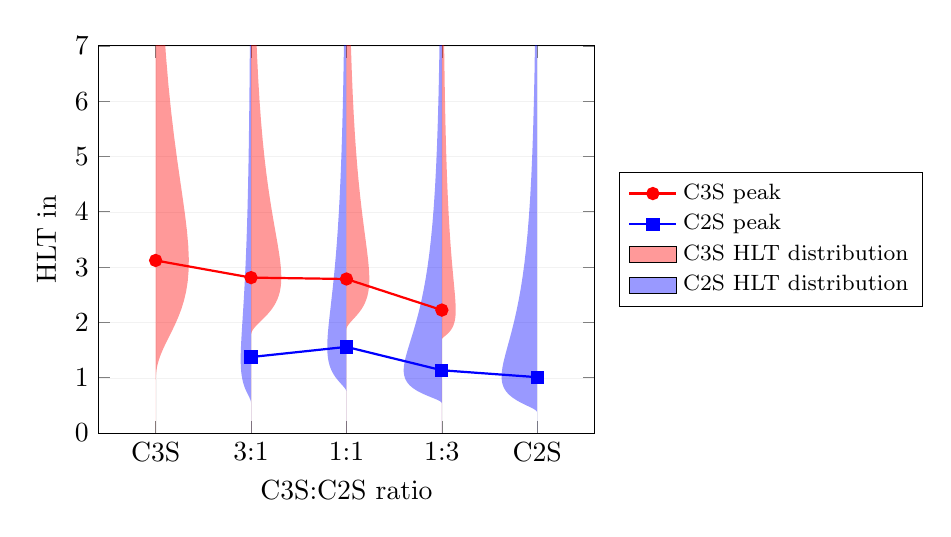
\begin{tikzpicture}
        \begin{axis}[
            width=0.65\textwidth,
            height=6.5cm,
			xlabel={\ac{C3S}:\ac{C2S} ratio},
            ylabel={\ac{HLT} in \unit{\micro\meter}},
            xmin=0, xmax=4,
            xtick={0,1,2,3,4},
            xticklabels={\ac{C3S}, 3:1, 1:1, 1:3, \ac{C2S}},
            enlarge x limits=0.15,
            ymin=0, ymax=7,
            ytick={0,1,...,7},
            grid=both,
            grid style={line width=.1pt, draw=gray!10},
            minor grid style={line width=.05pt, draw=gray!5},
            legend cell align={left},
            legend style={at={(1.05,.5)}, anchor=west, legend columns=1, font=\footnotesize},
        ]
            \pgfmathsetmacro{\vscale}{0.4}

            % pos 0: C3S (Right side only, using 28d pure phase data)
            \addplot [fill=red, fill opacity=0.4, draw=none, domain=-7:2, samples=100, forget plot] 
                ( {0 + \vscale * 0.869 * exp(-0.5 * ((\x - 0.887)/0.608)^2)}, {exp(\x) + 0.670} ) -- (0, 7) -- (0, 0) -- cycle;
            
            % pos 1: 3:1 (a_Belit=0.272, b=-0.206, c=1, d=0.523 | a_Alit=0.793, b=0.088, c=0.857, d=1.723)
            \addplot [fill=blue, fill opacity=0.4, draw=none, domain=-7:2, samples=100, forget plot] 
                ( {1 - \vscale * 0.272 * exp(-0.5 * ((\x - (-0.206))/1.000)^2)}, {exp(\x) + 0.523} ) -- (1, 7) -- (1, 0) -- cycle;
            \addplot [fill=red, fill opacity=0.4, draw=none, domain=-7:2, samples=100, forget plot] 
                ( {1 + \vscale * 0.793 * exp(-0.5 * ((\x - 0.088)/0.857)^2)}, {exp(\x) + 1.723} ) -- (1, 7) -- (1, 0) -- cycle;

            % pos 2: 1:1
            \addplot [fill=blue, fill opacity=0.4, draw=none, domain=-7:2, samples=100, forget plot] 
                ( {2 - \vscale * 0.503 * exp(-0.5 * ((\x - (-0.177))/1.000)^2)}, {exp(\x) + 0.720} ) -- (2, 7) -- (2, 0) -- cycle;
            \addplot [fill=red, fill opacity=0.4, draw=none, domain=-7:2, samples=100, forget plot] 
                ( {2 + \vscale * 0.599 * exp(-0.5 * ((\x - (-0.057))/0.940)^2)}, {exp(\x) + 1.840} ) -- (2, 7) -- (2, 0) -- cycle;

            % pos 3: 1:3
            \addplot [fill=blue, fill opacity=0.4, draw=none, domain=-7:2, samples=100, forget plot] 
                ( {3 - \vscale * 1.000 * exp(-0.5 * ((\x - (-0.491))/1.000)^2)}, {exp(\x) + 0.523} ) -- (3, 7) -- (3, 0) -- cycle;
            \addplot [fill=red, fill opacity=0.4, draw=none, domain=-7:2, samples=100, forget plot] 
                ( {3 + \vscale * 0.363 * exp(-0.5 * ((\x - (-0.626))/1.212)^2)}, {exp(\x) + 1.688} ) -- (3, 7) -- (3, 0) -- cycle;

            % pos 4: C2S (Left side only, using 28d pure phase data)
            \addplot [fill=blue, fill opacity=0.4, draw=none, domain=-7:2, samples=100, forget plot] 
                ( {4 - \vscale * 0.935 * exp(-0.5 * ((\x - (-0.404))/0.981)^2)}, {exp(\x) + 0.354} ) -- (4, 7) -- (4, 0) -- cycle;

            \addplot[color=red, mark=*, thick] coordinates {(0, 3.12) (1, 2.81) (2, 2.785) (3, 2.223)};
            \addlegendentry{\ac{C3S} peak};
            \addplot[color=blue, mark=square*, thick] coordinates {(1, 1.374) (2, 1.558) (3, 1.135) (4, 1.01)};
            \addlegendentry{\ac{C2S} peak};
            \addlegendimage{area legend, fill=red, fill opacity=0.4, draw=none}
            \addlegendentry{\ac{C3S} \ac{HLT} distribution}
            \addlegendimage{area legend, fill=blue, fill opacity=0.4, draw=none}
            \addlegendentry{\ac{C2S} \ac{HLT} distribution}
        \end{axis}
    \end{tikzpicture}
    \caption{
        Comparison of measured \ac{HLT} peak positions and their corresponding distributions of \ac{C3S}:\ac{C2S} mixtures after \qty{28}{\day} of hydration.
        The half-sided violin plots illustrate the fitted log-normal distributions (right: {\color{red}\ac{C3S}}, left: {\color{blue}\ac{C2S}}).
    }
    \label{fig:hydration-rim-mixture-results}
\end{figure}


In \zcref{fig:hydration-rim-mixture-results} it becomes apparent that \ac{C3S} reacts more slowly with increasing \ac{C2S} content, while \ac{C2S} reacts only slightly faster, if at all (raw data are listed in \zcref{tab:hlt_peak_measurements}).
As the proportion of a specific phase in the mixture decreases, its corresponding \ac{HLT} distribution tends to broaden, accompanied by a reduction in signal intensity.
Nevertheless, the peak for \ac{C3S} remains clearly visible across all mixtures due to its faster reaction kinetics.
This uncertainty may be caused by the following sources of error:
\begin{itemize}
	\item overlap/contact of the \ac{CSH} from \ac{C3S} and \ac{C2S},
	\item and filled \textsc{Hadley} grains with no contact to the actual hydrate layer around the grain, resulting in an overestimation and lower data density.
\end{itemize}

Manually reviewing the images furthermore reveals that the \textsc{Hadley} grain development is significantly more pronounced around \ac{C2S} grains in \ac{C3S}:\ac{C2S} mixtures (compare \zcref{fig:hadley2}).
This can cause a reduced \ac{HLT} measurement around \ac{C2S}.


\FloatBarrier
%\newpage
\section{Statistical analysis of the representativeness of the 2D images}

In this section, the images previously described in \zcref{sec:HLT_multi_phase} were used to assess the minimum area required to obtain a statistically relevant phase composition, using both the \ac{BC} and \ac{BG} methods.

The images were segmented via thresholding into four distinct phases: pores, \ac{CSH}, \ac{CH}, and clinker (see \zcref{fig:segmented_images}).
Although this segmentation approach produces erroneously segmented layers around clinker grains, which are consequently assigned to \ac{CH} instead of \ac{CSH} or the clinker phase, it is still considered adequate for estimating the overall phase composition.

\begin{figure}[htbp]

    \centering
	\includegraphics[height=.98\textheight]{hydrate-rim/segmented/overview.pdf}
	\caption{
        Segmented images of \ac{C3S}:\ac{C2S} mixtures after \num{7}, \num{14}, and \qty{28}{\day} of hydration. Red: {\color{red}\ac{CSH}}; yellow: {\color{orange}\ac{C3S}}; cyan: {\color{cyan}\ac{CH}}; black: pores.
    }
    \label{fig:segmented_images}
\end{figure}

\subsection{\Acl*{BC} method}

The result of the \ac{BC} method is a graph as shown in \zcref{fig:lit_box_count}.
The standard deviation $\sigma$ in \zcref{fig:lit_box_count_b} indicates the decreasing uncertainty as a larger area is analysed.
Compared to \zcref{fig:lit_box_growth_b}, $\sigma$ decreases continuously, since there is no location bias.

\begin{figure}[H]
    \centering
	\begin{subfigure}[t]{0.49\linewidth}
        \centering
      \begin{tikzpicture}
        \begin{axis}[
                xmin=0, xmax=1,
                ymin=0, ymax=80,
				xlabel={image area in \unit{\square\milli\meter}},
				ylabel={area fraction \unit{\percent}},
				xtick={0,.2,...,1},
                ytick={20,40,...,80},
                width=\linewidth,
				grid=major,
				grid style={line width=.1pt, draw=gray!10},
                xticklabel style={
                        /pgf/number format/fixed,
                        /pgf/number format/precision=1,
                        /pgf/number format/fixed zerofill,
                },
            ]

            %Pores
            \addplot+ [draw=none, no markers, name path=A,forget plot] table [x index=9, col sep=comma,y expr={\thisrowno{1}-\thisrowno{2}}, ] {figures/literature/C3S_28d_box_count.csv};
            \addplot+ [draw=none, no markers, name path=B,forget plot] table [x index=9, col sep=comma,y expr={\thisrowno{1}+\thisrowno{2}}, ] {figures/literature/C3S_28d_box_count.csv};

            \addplot [fill=black, fill opacity=0.2,forget plot] fill between [of=A and B];

            \addplot [ mark=none, black, opacity=0.5 ] table [x index=9, y index=1, col sep=comma] {figures/literature/C3S_28d_box_count.csv};
            %\addlegendentry{pores};

            %CSH
            \addplot+ [draw=none, no markers, name path=A,forget plot] table [x index=9, col sep=comma,y expr={\thisrowno{3}-\thisrowno{4}}, ] {figures/literature/C3S_28d_box_count.csv};
            \addplot+ [draw=none, no markers, name path=B,forget plot] table [x index=9, col sep=comma,y expr={\thisrowno{3}+\thisrowno{4}}, ] {figures/literature/C3S_28d_box_count.csv};

            \addplot [fill=red, fill opacity=0.2,forget plot] fill between [of=A and B];

            \addplot [ mark=none, red, opacity=0.5 ] table [x index=9, y index=3, col sep=comma] {figures/literature/C3S_28d_box_count.csv};
            %\addlegendentry{\ac{CSH}};

            %CH
            \addplot+ [draw=none, no markers, name path=A,forget plot] table [x index=9, col sep=comma,y expr={\thisrowno{5}-\thisrowno{6}}, ] {figures/literature/C3S_28d_box_count.csv};
            \addplot+ [draw=none, no markers, name path=B,forget plot] table [x index=9, col sep=comma,y expr={\thisrowno{5}+\thisrowno{6}}, ] {figures/literature/C3S_28d_box_count.csv};

            \addplot [fill=cyan, fill opacity=0.2,forget plot] fill between [of=A and B];

            \addplot [ mark=none, cyan, opacity=0.5 ] table [x index=9, y index=5, col sep=comma] {figures/literature/C3S_28d_box_count.csv};
            %\addlegendentry{\ac{CH}};

            %alite
            \addplot+ [draw=none, no markers, name path=A,forget plot] table [x index=9, col sep=comma,y expr={\thisrowno{7}-\thisrowno{8}}, ] {figures/literature/C3S_28d_box_count.csv};
            \addplot+ [draw=none, no markers, name path=B,forget plot] table [x index=9, col sep=comma,y expr={\thisrowno{7}+\thisrowno{8}}, ] {figures/literature/C3S_28d_box_count.csv};

            \addplot [fill=orange, fill opacity=0.2,forget plot] fill between [of=A and B];

            \addplot [ mark=none, orange, opacity=0.5 ] table [x index=9, y index=7, col sep=comma] {figures/literature/C3S_28d_box_count.csv};
            %\addlegendentry{alite};
        \end{axis}
      \end{tikzpicture}
      \caption{Phase composition statistics.}
      \label{fig:lit_box_count_a}
    \end{subfigure}%
    \hfill%
	\begin{subfigure}[t]{0.49\linewidth}
      \centering
      \begin{tikzpicture}
		\begin{axis}[
            width=\linewidth,
            xmin=0, xmax=1,
            ymin=0, ymax=10,
            xlabel={image area in \unit{\square\milli\meter}},
            legend style={at={(.98,.98)},anchor=north east},
            ylabel={standard deviation $\sigma$ in \unit{\percent}},
            xtick={0,.2,...,1},
            ytick={2,4,...,10},
            ylabel near ticks, yticklabel pos=right,
            grid=major,
            grid style={line width=.1pt, draw=gray!10},
            xticklabel style={
                    /pgf/number format/fixed,
                    /pgf/number format/precision=1,
                    /pgf/number format/fixed zerofill,
            },
		  ]
          \addplot[black, smooth, tension=0.5, no markers] table [x index=9, col sep=comma,y index=2] {figures/literature/C3S_28d_box_count.csv};

          \addplot[red, smooth, tension=0.5, no markers] table [x index=9, col sep=comma,y index=4] {figures/literature/C3S_28d_box_count.csv};

          \addplot[cyan, smooth, tension=0.5, no markers] table [x index=9, col sep=comma,y index=6] {figures/literature/C3S_28d_box_count.csv};

          \addplot[orange, smooth, tension=0.5, no markers] table [x index=9, col sep=comma,y index=8] {figures/literature/C3S_28d_box_count.csv};
          \addlegendentry{pores};
          \addlegendentry{\ac{CSH}};
          \addlegendentry{\ac{CH}};
          \addlegendentry{\ac{C3S}};
        \end{axis}
      \end{tikzpicture}
      \caption{Standard deviation of the phase composition.}
      \label{fig:lit_box_count_b}
    \end{subfigure}
    \caption{
        Results of the \ac{BC} as explained in \cite{mouret.2001,hlavacek.2015} and the respective standard deviations (right) after the selection of up to \num{100} random tiles.
    }
    \label{fig:lit_box_count}
\end{figure}

Therefore, the $\sigma$ can directly be used to define the minimum required area.
This point is reached if $\sigma$ is below \qty{2}{\percent}.

Since the phase composition of each image section can be calculated before the randomisation, the \ac{BC} method is fairly fast, even for many repeated experiments.
Furthermore, it is insensitive to the influence of larger inhomogeneities, such as the rather large \ac{CH} areas or occasionally occurring air voids.


\subsection{\Acl*{BG} method}

\zcref{fig:lit_box_growth} shows the result of the \ac{BG} method applied to an image of \qty{28}{\day} hydrated \ac{C3S}.
This image must be segmented beforehand into pores, unhydrated \ac{C3S}, \ac{CH}, and \ac{CSH}.
The standard deviation in \zcref{fig:lit_box_growth_b} indicates the decreasing uncertainty as a larger area is analysed.

\begin{figure}[H]
    \centering
    \begin{subfigure}[t]{0.49\linewidth}
      \begin{tikzpicture}
        \begin{axis}[
                xmin=0, xmax=1,
                ymin=0, ymax=80,
                width=\linewidth,
                xlabel={image area in \unit{\square\milli\meter}},
                ylabel={phase amount \unit{\percent}},
                xtick={0,0.2,...,1},
                ytick={20,40,...,80},
				grid=major,
				grid style={line width=.1pt, draw=gray!10},
                xticklabel style={
                        /pgf/number format/fixed,
                        /pgf/number format/precision=1,
                        /pgf/number format/fixed zerofill,
                },
            ]

            %Pores
            \addplot+ [draw=none, no markers, name path=A,forget plot] table [x index=9, col sep=comma,y expr={\thisrowno{1}-\thisrowno{2}}, ] {figures/literature/C3S_28d_area_growth.csv};
            \addplot+ [draw=none, no markers, name path=B,forget plot] table [x index=9, col sep=comma,y expr={\thisrowno{1}+\thisrowno{2}}, ] {figures/literature/C3S_28d_area_growth.csv};

            \addplot [fill=black, fill opacity=0.2,forget plot] fill between [of=A and B];

            \addplot [ mark=none, black, opacity=0.5 ] table [x index=9, y index=1, col sep=comma] {figures/literature/C3S_28d_area_growth.csv};
            %\addlegendentry{pores};

            %CSH
            \addplot+ [draw=none, no markers, name path=A,forget plot] table [x index=9, col sep=comma,y expr={\thisrowno{3}-\thisrowno{4}}, filter discard warning=false ] {figures/literature/C3S_28d_area_growth.csv};
            \addplot+ [draw=none, no markers, name path=B,forget plot] table [x index=9, col sep=comma,y expr={\thisrowno{3}+\thisrowno{4}}, filter discard warning=false ] {figures/literature/C3S_28d_area_growth.csv};

            \addplot [fill=red, fill opacity=0.2,forget plot] fill between [of=A and B];

            \addplot [ mark=none, red, opacity=0.5 ] table [x index=9, y index=3, col sep=comma, filter discard warning=false] {figures/literature/C3S_28d_area_growth.csv};
            %\addlegendentry{\ac{CSH}};

            %CH
            \addplot+ [draw=none, no markers, name path=A,forget plot] table [x index=9, col sep=comma,y expr={\thisrowno{5}-\thisrowno{6}}, filter discard warning=false ] {figures/literature/C3S_28d_area_growth.csv};
            \addplot+ [draw=none, no markers, name path=B,forget plot] table [x index=9, col sep=comma,y expr={\thisrowno{5}+\thisrowno{6}}, filter discard warning=false ] {figures/literature/C3S_28d_area_growth.csv};

            \addplot [fill=cyan, fill opacity=0.2,forget plot] fill between [of=A and B];

            \addplot [ mark=none, cyan, opacity=0.5 ] table [x index=9, y index=5, col sep=comma, filter discard warning=false] {figures/literature/C3S_28d_area_growth.csv};
            %\addlegendentry{\ac{CH}};

            %alite
            \addplot+ [draw=none, no markers, name path=A,forget plot] table [x index=9, col sep=comma,y expr={\thisrowno{7}-\thisrowno{8}}, filter discard warning=false ] {figures/literature/C3S_28d_area_growth.csv};
            \addplot+ [draw=none, no markers, name path=B,forget plot] table [x index=9, col sep=comma,y expr={\thisrowno{7}+\thisrowno{8}}, filter discard warning=false ] {figures/literature/C3S_28d_area_growth.csv};

            \addplot [fill=orange, fill opacity=0.2,forget plot] fill between [of=A and B];

            \addplot [ mark=none, orange, opacity=0.5 ] table [x index=9, y index=7, col sep=comma, filter discard warning=false] {figures/literature/C3S_28d_area_growth.csv};
            %\addlegendentry{alite};
        \end{axis}
      \end{tikzpicture}
      \caption{Phase composition.}
      \label{fig:lit_box_growth_a}
    \end{subfigure}
    \hfill%
    \begin{subfigure}[t]{0.49\linewidth}
      \begin{tikzpicture}
		\begin{axis}[%red,
            xmin=0, xmax=1,
            ymin=0, ymax=10,
            width=\linewidth,
            legend style={at={(.98,.98)},anchor=north east},
            %axis y line=right,
            ylabel near ticks, yticklabel pos=right,
			xlabel={image area in \unit{\square\milli\meter}},
			ylabel={standard deviation $\sigma$ in \unit{\percent}},
            xtick={0,0.2,...,1},
            ytick={2,4,...,10},
            grid=major,
            grid style={line width=.1pt, draw=gray!10},
            xticklabel style={
                    /pgf/number format/fixed,
                    /pgf/number format/precision=1,
                    /pgf/number format/fixed zerofill,
            },
		  ]
          \addplot[black, smooth, tension=0.2, no markers] table [x index=9, col sep=comma,y index=2, filter discard warning=false] {figures/literature/C3S_28d_area_growth.csv};

          \addplot[red, smooth, tension=0.2, no markers] table [x index=9, col sep=comma,y index=4, filter discard warning=false] {figures/literature/C3S_28d_area_growth.csv};

          \addplot[cyan, smooth, tension=0.2, no markers] table [x index=9, col sep=comma,y index=6, filter discard warning=false] {figures/literature/C3S_28d_area_growth.csv};

          \addplot[orange, smooth, tension=0.2, no markers] table [x index=9, col sep=comma,y index=8, filter discard warning=false] {figures/literature/C3S_28d_area_growth.csv};

          \addlegendentry{pores};
          \addlegendentry{\ac{CSH}};
          \addlegendentry{\ac{CH}};
          \addlegendentry{\ac{C3S}};

        \end{axis}
      \end{tikzpicture}
      \caption{Standard deviation of the phase composition.}
      \label{fig:lit_box_growth_b}
    \end{subfigure}
    \caption{
        Example of the results of the \ac{BG} method as explained in \cite{bosl.1998,kameda.2006} and the respective standard deviations for \num{100} random starting points.
    }
    \label{fig:lit_box_growth}
\end{figure}

In contrast to the \ac{BC} method, the standard deviation of the \ac{BG} method decreases unsteadily.
This is caused by the fact that the position of the random growth point is limited.
Since the location of larger phases like pores or \ac{CH} does not change in the image, their position can have a significant influence. 
Even the randomised starting point cannot remove the bias if only a single large image is used for this technique.
Nevertheless, the standard deviation is below \qty{2}{\percent} at \qty{0.1}{\square\milli\meter}.
However, due to this effect, the deviation from the phase measurement of the whole specimen can still be more than \qty{2}{\percent}.
Due to this unsteadiness, $\sigma_{\text{BG}}$ was not directly set to the measured $\sigma$.
Instead, the method-specific standard deviation $\sigma_{\text{BG}}$ is defined as the absolute difference between the phase concentration of the whole image ($\phi_{\text{img}}$) and the phase concentration in the current image area ($\phi_{\text{area}}$), plus the absolute value of the standard deviation ($\sigma$) of the current image area:

\begin{equation}
    \sigma_{\text{BG}} = \lvert\phi_{\text{img}} - \phi_{\text{area}} \rvert + \lvert\sigma\rvert
    \label{eq:phase_difference}
\end{equation}

The largest minimum required area is therefore reached if $\sigma_{\text{BG}}$ is below \qty{2}{\percent}.

Since the phase composition must be recalculated for each repeated experiment, this method is significantly slower than the \ac{BC} method.


\subsection{Evaluation}

The minimum required area for a standard deviation $\sigma$ of <\,\qty{2}{\percent} was calculated for each phase.

The largest minimum required area can be found in the pore and clinker phases, which are plotted in \zcref{fig:box_statistics_clinker}.
The hydrate phases \ac{CSH} and \ac{CH} showed a significantly lower minimum required area (see \zcref{fig:box_statistics_ch}).
The results are also listed in \zcref{tab:convergence_area_box_cnt, tab:convergence_area_box_growth}.

\begin{figure}[htb]
    \centering
    \begin{subfigure}[b]{0.49\textwidth}
        \centering
        \begin{tikzpicture}
            \begin{axis}[
                ybar,
                ymin=0, ymax=1.3,
                ylabel={min. area in \unit{\milli\meter\squared}},
                symbolic x coords={1:0, 3:1, 1:1, 1:3, 0:1},
                xtick=data,
                xlabel={\ac{C3S}:\ac{C2S} ratio},
                bar width=8pt,
                enlarge x limits=0.2,
                %legend style={legend pos=north, legend columns=1}, % NEU: Legende oben
                width=\textwidth,
                height=6cm,
                y tick label style={
                    /pgf/number format/fixed,
                    /pgf/number format/fixed zerofill,
                    /pgf/number format/precision=1
                },
            ]
                % 7d Pores Data (Reihenfolge: 1:0, 3:1, 1:1, 1:3, 0:1)
                \addplot[fill=yellow, draw opacity=0, bar shift=-9pt] coordinates {
                    (1:0, 0.03165) (3:1, 0.03617) (1:1, 0.02707) (1:3, 0.02110) (0:1, 0.02411)
                };
                \addlegendentry{\qty{7}{\day}}

                % 14d Pores Data
                \addplot[fill=orange, draw opacity=0] coordinates {
                    (1:0, 0.03165) (3:1, 0.02101) (1:1, 0.15633) (1:3, 0.02261) (0:1, 0.00904)
                };
                \addlegendentry{\qty{14}{\day}}

                % 28d Pores Data
                \addplot[fill=red, draw opacity=0, bar shift=9pt] coordinates {
                    (1:0, 0.01055) (3:1, 0.07820) (1:1, 0.01808) (1:3, 0.00546) (0:1, 0.01808)
                };
                \addlegendentry{\qty{28}{\day}}
            \end{axis}
        \end{tikzpicture}
        \caption{
            Pores, \ac{BC} method.
        }
        \label{fig:convergence_pores}
    \end{subfigure}
    \hfill
    \begin{subfigure}[b]{0.49\textwidth}
        \centering
        \begin{tikzpicture}
            \begin{axis}[
                ybar,
                ymin=0, ymax=1.3,
                ylabel={min. area in \unit{\milli\meter\squared}},
                symbolic x coords={1:0, 3:1, 1:1, 1:3, 0:1},
                xtick=data,
                xlabel={\ac{C3S}:\ac{C2S} ratio},
                bar width=8pt,
                enlarge x limits=0.2,
                %legend style={legend pos=north, legend columns=1}, % NEU: Legende oben
                width=\textwidth,
                height=6cm,
                ylabel near ticks,
                yticklabel pos=right,
                y tick label style={
                    /pgf/number format/fixed,
                    /pgf/number format/fixed zerofill,
                    /pgf/number format/precision=1
                },
            ]
                % 7d Pores Data (Reihenfolge: 1:0, 3:1, 1:1, 1:3, 0:1)
                \addplot[fill=green, draw opacity=0, bar shift=-9pt] coordinates {
                    (1:0, 0.144934) (3:1, 0.065734) (1:1, 0.101282) (1:3, 0.019552) (0:1, 0.262979)
                };
                \addlegendentry{\qty{7}{\day}}

                % 14d Pores Data
                \addplot[fill=cyan, draw opacity=0] coordinates {
                    (1:0, 0.058000) (3:1, 0.065431) (1:1, 1.248485) (1:3, 0.029220) (0:1, 0.182607)
                };
                \addlegendentry{\qty{14}{\day}}

                % 28d Pores Data
                \addplot[fill=blue, draw opacity=0, bar shift=9pt] coordinates {
                    (1:0, 0.026615) (3:1, 0.466620) (1:1, 0.054304) (1:3, 0.034310) (0:1, 0.031932)
                };
                \addlegendentry{\qty{28}{\day}}
            \end{axis}
        \end{tikzpicture}
        \caption{
            Pores, \ac{BG} method.
        }
        \label{fig:areagrowth_pores}
    \end{subfigure}
    
    \begin{subfigure}[b]{0.49\textwidth}
        \centering
        \begin{tikzpicture}
            \begin{axis}[
                ybar,
                ymin=0, ymax=1.3, % NEU: Angepasst an max(0.4, 1.1)
                ylabel={min. area in \unit{\milli\meter\squared}},
                symbolic x coords={1:0, 3:1, 1:1, 1:3, 0:1},
                xtick=data,
                xlabel={\ac{C3S}:\ac{C2S} ratio},
                bar width=8pt,
                enlarge x limits=0.2,
                %legend style={legend pos=north, legend columns=1}, % NEU
                width=\textwidth, % NEU
                height=6cm,
                y tick label style={
                    /pgf/number format/fixed,
                    /pgf/number format/fixed zerofill,
                    /pgf/number format/precision=1
                },
            ]
                % 7d clinker Data
                \addplot[fill=yellow, draw opacity=0, bar shift=-9pt] coordinates {
                    (1:0, 0.04522) (3:1, 0.04974) (1:1, 0.04361) (1:3, 0.01356) (0:1, 0.00602)
                };
                \addlegendentry{\qty{7}{\day}}

                % 14d clinker Data
                \addplot[fill=orange, draw opacity=0] coordinates {
                    (1:0, 0.01356) (3:1, 0.03752) (1:1, 0.15633) (1:3, 0.01808) (0:1, 0.00904)
                };
                \addlegendentry{\qty{14}{\day}}

                % 28d clinker Data
                \addplot[fill=red, draw opacity=0, bar shift=9pt] coordinates {
                    (1:0, 0.02562) (3:1, 0.30678) (1:1, 0.14470) (1:3, 0.01966) (0:1, 0.01055)
                };
                \addlegendentry{\qty{28}{\day}}
            \end{axis}
        \end{tikzpicture}
        \caption{
            Clinker, \ac{BC} method.
        }
        \label{fig:convergence_clinker}
    \end{subfigure}
    \hfill
    \begin{subfigure}[b]{0.49\textwidth}
        \centering
        \begin{tikzpicture}
            \begin{axis}[
                ybar,
                ymin=0, ymax=1.3,
                ylabel={min. area in \unit{\milli\meter\squared}},
                symbolic x coords={1:0, 3:1, 1:1, 1:3, 0:1},
                xtick=data,
                xlabel={\ac{C3S}:\ac{C2S} ratio},
                bar width=8pt,
                enlarge x limits=0.2,
                %legend style={legend pos=north, legend columns=1}, % NEU
                width=\textwidth,
                height=6cm,
                ylabel near ticks,
                yticklabel pos=right,
                y tick label style={
                    /pgf/number format/fixed,
                    /pgf/number format/fixed zerofill,
                    /pgf/number format/precision=1
                },
                %yticklabel={\ifdim\tick pt=0pt 0 \else\pgfmathprintnumber{\tick}\fi}
            ]
                % 7d clinker Data
                \addplot[fill=green, draw opacity=0, bar shift=-9pt] coordinates {
                    (1:0, 0.054324) (3:1, 0.078231) (1:1, 0.188929) (1:3, 0.015454) (0:1, 0.050768)
                };
                \addlegendentry{\qty{7}{\day}}

                % 14d clinker Data
                \addplot[fill=cyan, draw opacity=0] coordinates {
                    (1:0, 0.047315) (3:1, 0.162460) (1:1, 0.138721) (1:3, 0.024144) (0:1, 0.106486)
                };
                \addlegendentry{\qty{14}{\day}}

                % 28d clinker Data
                \addplot[fill=blue, draw opacity=0, bar shift=9pt] coordinates {
                    (1:0, 0.101484) (3:1, 0.810745) (1:1, 1.051917) (1:3, 0.113844) (0:1, 0.024144)
                };
                \addlegendentry{\qty{28}{\day}}
            \end{axis}
        \end{tikzpicture}
        \caption{
            Clinker, \ac{BG} method.
        }
        \label{fig:areagrowth_clinker}
    \end{subfigure}
    \caption{
        Comparison of the minimum required area required to obtain the pore area fraction (top row) and the clinker area fraction (bottom row) with a standard deviation $\sigma$ of <\,\qty{2}{\percent}.
        The \ac{BC} and \ac{BG} methods were applied to images of \ac{C3S}:\ac{C2S} mixtures, hydrated for \num{7}, \num{14} and \qty{28}{\day}.
    }
    \label{fig:box_statistics_clinker}
\end{figure}

The plots indicate no apparent correlation between the minimum required area and either the \ac{C3S}:\ac{C2S} ratio or the hydration time.
The \ac{BG} method consistently yields a larger required area than the \ac{BC} method.

A visual comparison between the images (\zcref{fig:segmented_images}) and the results reveals that the \ac{BG} method is highly sensitive to irregularities, such as air voids or \ac{CH} patches.
As these larger features are not uniformly distributed within the image, they can have a significant influence on the standard deviation.
Furthermore, given that the initial starting area is constrained to one-fifth of the central image area, it is probable that some of these large features are included in all or most of the experiments.
This directly causes the unsteady decrease observed in \zcref{fig:lit_box_growth_b}.

In summary, images of hydrated \ac{C3S}:\ac{C2S} paste exhibiting considerable inhomogeneities (e.g. air voids) require significantly larger areas (more than \qty{1.4}{\milli\meter\squared}) to achieve statistical representativeness compared to highly homogeneous specimens, for which an area exceeding \qty{0.3}{\milli\meter\squared} is sufficient.
Moreover, this dependence on feature size (the larger the feature, the larger the image) demonstrates that an analysis of statistical representativeness must be conducted on an image-by-image basis and depends on the specimen type.
For comparison, \textcite{stutzman.2004} determined that areas larger than \qty{0.2}{\milli\meter\squared} are sufficient for statistical representativeness when analysing polished cement clinker.

Furthermore, there is a significant subjective influence of the \ac{SEM} operator, which can hardly be avoided.
For example, to acquire the large images evaluated in this study, only the best areas with few pores and irregularities were manually selected from the specimen surface.
\textcite{kameda.2006} pointed out that the data fluctuation of the measured porosity and permeability using this method becomes negligible when `\textit{the cube size exceeds four grain radii}'.
 